بازی
fair-cost-sharing
:
یک شبکه داریم. افراد مختلف در راس‌های مختلف شبکه هستند و می‌خواهند به مقصد‌های مختلف بروند. هر یال
$e$
یک هزینه
$c_e$
دارد که باید بین افرادی که از آن یال استفاده می‌کنند، به طور مساوی تقسیم شود. هر کسی می‌خواهد هزینه خود را کمینه کند.

برای مثال، این شبکه را در نظر بگیرید:
\begin{center}
    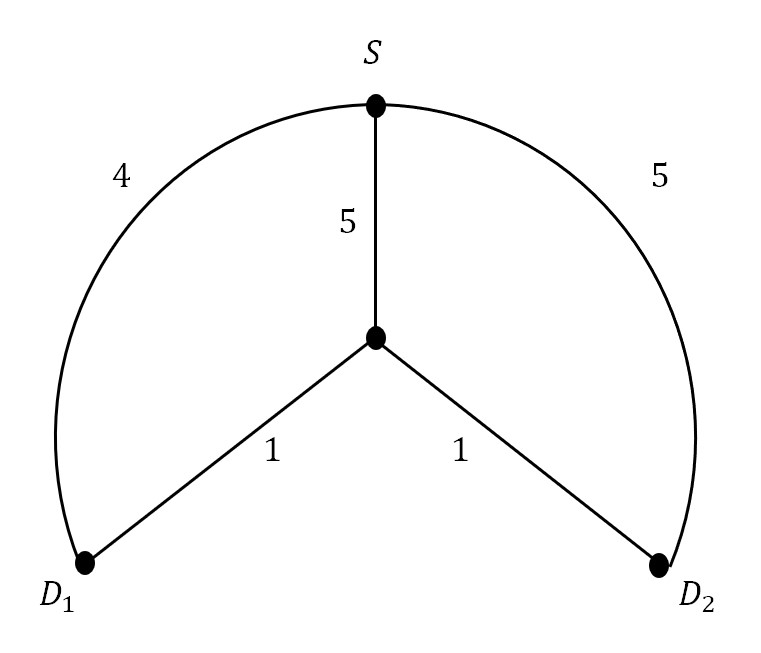
\includegraphics[width=0.35\linewidth]{pics/image6}
\end{center}
در این بازی، ۲ نفر می‌خواهند از راس
$S$
به
$D_1$
و
$D_2$
بروند. این بازی ۲ تعادل دارد: اولی از ۴ و دومی از ۵ یا هر دو از مسیر ۵ و ۱ با هم بروند. مشخصا در اینجا تعادل دوم مطلوب‌تر است.

آیا
fair-cost-sharing
به طور کلی یک بازی پتانسیلی است؟